\documentclass[12pt]{article}

\usepackage{algorithm}
\usepackage{algorithmicx}
\usepackage{algpseudocode}
\usepackage{amsmath}
\usepackage{amsthm}
\usepackage{tikz}
\usetikzlibrary{arrows,automata}

\title{EECS 477 HW3}
\author{Andrew Mason}

\begin{document}
\maketitle

\begin{enumerate}
  % #1
  \item
    \begin{enumerate}
      \item
        \begin{itemize}
          \item First, put all lower bounds to 0.\\
            \begin{tabular}{|r|c|c|}
              \hline
              Node & $b_i$ \\\hline
              a & 15 \\ \hline
              b & 10 \\ \hline
              c & -20 \\ \hline
              d & -5 \\ \hline
              e & 0 \\ \hline
            \end{tabular}
            \begin{tabular}{|r|c|c|c|}
              \hline
              Arc & $c$ & $u$ \\ \hline
              (a, b) & 4 & $\infty$ \\ \hline
              (a, c) & 6 & $\infty$ \\ \hline
              (b, c) & -2 & 25 \\ \hline
              (b, e) & 5 & 10 \\ \hline
              (c, d) & -3 & 5 \\ \hline
              (e, d) & 2 & $\infty$ \\ \hline
            \end{tabular}
          \item Next, reverse arcs with negative costs.\\
            \begin{tabular}{|r|c|c|}
              \hline
              Node & $b_i$ \\\hline
              a & 15 \\ \hline
              b & -15 \\ \hline
              c & 0 \\ \hline
              d & 0 \\ \hline
              e & 0 \\ \hline
            \end{tabular}
            \begin{tabular}{|r|c|c|c|}
              \hline
              Arc & $c$ & $u$ \\ \hline
              (a, b) & 4 & $\infty$ \\ \hline
              (a, c) & 6 & $\infty$ \\ \hline
              (c, b) & 2 & 25 \\ \hline
              (b, e) & 5 & 10 \\ \hline
              (d, c) & 3 & 5 \\ \hline
              (e, d) & 2 & $\infty$ \\ \hline
            \end{tabular}
          \item Finally, put all upper bounds to $\infty$.\\
            \begin{tabular}{|r|c|c|}
              \hline
              Node & $b_i$ \\\hline
              a & 15 \\ \hline
              b & 10 \\ \hline
              c & 5 \\ \hline
              d & 0 \\ \hline
              e & 10 \\ \hline
              i & -10 \\ \hline
              j & -5 \\ \hline
              k & -25 \\ \hline
            \end{tabular}
            \begin{tabular}{|r|c|c|}
              \hline
              Arc & $c$ \\ \hline
              (a, b) & 4 \\ \hline
              (a, c) & 6 \\ \hline
              (c, k) & 2 \\ \hline
              (b, k) & 0 \\ \hline
              (b, i) & 5 \\ \hline
              (e, i) & 0 \\ \hline
              (d, j) & 3 \\ \hline
              (c, j) & 0 \\ \hline
              (e, d) & 2 \\ \hline
            \end{tabular}
        \end{itemize}
      \item
        Sending 20 units of flow along $(a,b)$ satisfies the supply constraint
        of $a$, and the lower bound constraint of $(a, b)$. Now, sending 25
        units of flow along $(b,c)$ yields a net outgoing flow for $b$ of 5,
        satisfying the supply constraint of $b$. Additionally, 25 is within the
        upper bound for $(b,c)$, so we have not yet violated any constraints.
        Finally, sending 10 units of flow along $(c,d)$ results in a net
        outgoing flow of -15 for $c$, and a net outgoing flow of -10 for $d$,
        so both nodes have their supplies satisfied. Additionally, 10 is within
        the upper bound for $(c,d)$, so this does not violate the upper bound
        of the arc. $e$ sees no flow, but its supply constraint is 0, so this
        is fine. Also, all of the arcs that had no flow move across them have
        lower bounds of 0, so the flow is feasible.\\

        The residual network is:\\
          \begin{center}
            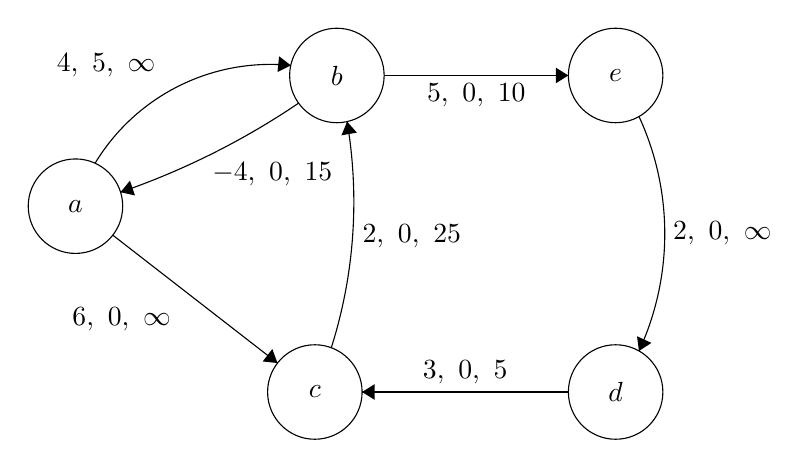
\begin{tikzpicture}[scale=0.2]
              \tikzstyle{every node}+=[inner sep=0pt]
              \draw [black] (11.2,-18.2) circle (3);
              \draw (11.2,-18.2) node {$a$};
              \draw [black] (27.8,-9.9) circle (3);
              \draw (27.8,-9.9) node {$b$};
              \draw [black] (26.4,-30) circle (3);
              \draw (26.4,-30) node {$c$};
              \draw [black] (45.5,-9.9) circle (3);
              \draw (45.5,-9.9) node {$e$};
              \draw [black] (45.5,-30) circle (3);
              \draw (45.5,-30) node {$d$};
              \draw [black] (13.57,-20.04) -- (24.03,-28.16);
              \fill [black] (24.03,-28.16) -- (23.7,-27.27) -- (23.09,-28.06);
              \draw (14.13,-24.6) node [below] {$6,\mbox{ }0,\mbox{ }\infty$};
              \draw [black] (42.5,-30) -- (29.4,-30);
              \fill [black] (29.4,-30) -- (30.2,-30.5) -- (30.2,-29.5);
              \draw (35.95,-29.5) node [above] {$3,\mbox{ }0,\mbox{ }5$};
              \draw [black] (12.443,-15.477) arc (148.85059:84.27952:13.011);
              \fill [black] (24.88,-9.26) -- (24.13,-8.68) -- (24.03,-9.68);
              \draw (13.14,-10.05) node [above] {$4,\mbox{ }5,\mbox{ }\infty$};
              \draw [black] (25.369,-11.658) arc (-55.9088:-70.96109:48.25);
              \fill [black] (14.06,-17.31) -- (14.98,-17.52) -- (14.66,-16.58);
              \draw (23.7,-15.37) node [below] {$-4,\mbox{ }0,\mbox{ }15$};
              \draw [black] (30.8,-9.9) -- (42.5,-9.9);
              \fill [black] (42.5,-9.9) -- (41.7,-9.4) -- (41.7,-10.4);
              \draw (36.65,-10.4) node [below] {$5,\mbox{ }0,\mbox{ }10$};
              \draw [black] (46.983,-12.504) arc (24.81077:-24.81077:17.745);
              \fill [black] (46.98,-27.4) -- (47.77,-26.88) -- (46.86,-26.46);
              \draw (49.12,-19.95) node [right] {$2,\mbox{ }0,\mbox{ }\infty$};
              \draw [black] (28.446,-12.828) arc (9.62353:-17.59216:30.593);
              \fill [black] (28.45,-12.83) -- (28.09,-13.7) -- (29.07,-13.53);
              \draw (29.4,-20.11) node [right] {$2,\mbox{ }0,\mbox{ }25$};
            \end{tikzpicture}
          \end{center}
    \end{enumerate}
  % #2
  \item
    One such network is:\\
    \begin{center}
      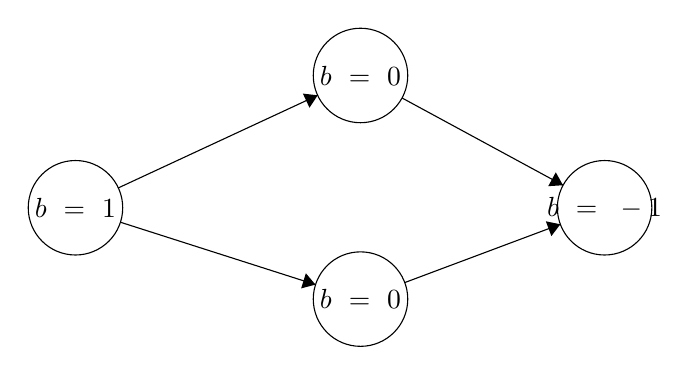
\begin{tikzpicture}[scale=0.2]
        \tikzstyle{every node}+=[inner sep=0pt]
        \draw [black] (19.6,-27.1) circle (3);
        \draw (19.6,-27.1) node {$b\mbox{ }=\mbox{ }1$};
        \draw [black] (37.7,-18.7) circle (3);
        \draw (37.7,-18.7) node {$b\mbox{ }=\mbox{ }0$};
        \draw [black] (37.7,-32.9) circle (3);
        \draw (37.7,-32.9) node {$b\mbox{ }=\mbox{ }0$};
        \draw [black] (53.2,-27.1) circle (3);
        \draw (53.2,-27.1) node {$b\mbox{ }=\mbox{ }-1$};
        \draw [black] (22.32,-25.84) -- (34.98,-19.96);
        \fill [black] (34.98,-19.96) -- (34.04,-19.85) -- (34.46,-20.75);
        \draw [black] (40.34,-20.13) -- (50.56,-25.67);
        \fill [black] (50.56,-25.67) -- (50.1,-24.85) -- (49.62,-25.73);
        \draw [black] (22.46,-28.02) -- (34.84,-31.98);
        \fill [black] (34.84,-31.98) -- (34.23,-31.26) -- (33.93,-32.22);
        \draw [black] (40.51,-31.85) -- (50.39,-28.15);
        \fill [black] (50.39,-28.15) -- (49.47,-27.96) -- (49.82,-28.9);
      \end{tikzpicture}
    \end{center}

    All costs are 1, lower bounds 0 and upper bounds $\infty$. An
    optimal fractional solution is to send $\frac{1}{2}$ of a unit
    of flow along the upper path, and $\frac{1}{2}$ of a unit of flaw
    along the lower path.\\
  % #3
  \item
    The MCNF problem in number 1 can be formulated as the following linear program:\\
    \begin{equation}
      \begin{split}
        \text{min}\ &4x_{ab}+6x_{ac}-2x_{bc}+5x_{be}-3x_{cd}+2x_{ed}\\
        \text{s.t.}\ &x_{ab}+x_{ac}=20\\
        &-x_{ab}+x_{bc}+x_{be}=5\\
        &-x_{ac}-x_{bc}+x_{cd}=-15\\
        &-x_{cd}-x_{ed}=-10\\
        &-x_{be}+x_{ed}=0\\
        &x_{ab}\geq5\\
        &-x_{bc}\geq-25\\
        &-x_{be}\geq-10\\
        &x_{cd}\geq5\\
        &-x_{cd}\geq-10\\
        &x_{ac},x_{bc},x_{be},x_{ed}\geq0\\
      \end{split}
    \end{equation}

    The dual is then:\\
    \begin{equation}
      \begin{split}
        \text{max}\ &20\pi_1+5\pi_2-15\pi_3-10\pi_4+0\pi_5+5\alpha_1-20\alpha_2-10\alpha_3+5\alpha_4-10\alpha_5\\
        \text{s.t.}\ &\pi_1-\pi_2+\alpha_1\leq4\\
        &\pi_1-\pi_3\leq6\\
        &\pi_2-\pi_3-\alpha_2\leq-2\\
        &\pi_2-\pi_5-\alpha_3\leq5\\
        &\pi_3-\pi_4+\alpha_4-\alpha_5\leq-3\\
        &-\pi_4+\pi_5\leq2\\
        &\alpha_i\geq0,i=1\ldots5\\
        &\pi_i\ \text{unrestricted},i=1\ldots5\\
      \end{split}
    \end{equation}

    So the complementary slackness conditions are:\\
    \begin{equation}
      \begin{split}
        x_{ab}=0\ &\text{or}\ \pi_1-\pi_2+\alpha_1=4\\
        x_{ac}=0\ &\text{or}\ \pi_1-\pi_3=6\\
        x_{bc}=0\ &\text{or}\ \pi_2-\pi_3-\alpha_2=-2\\
        x_{be}=0\ &\text{or}\ \pi_2-\pi_5-\alpha_3=5\\
        x_{cd}=0\ &\text{or}\ \pi_3-\pi_4+\alpha_4-\alpha_5=-3\\
        x_{ed}=0\ &\text{or}\ -\pi_4+\pi_5=2\\
        \pi_1=0\ &\text{or}\ x_{ab}+x_{ac}=20\\
        \pi_2=0\ &\text{or}\ -x_{ab}+x_{bc}+x_{be}=5\\
        \pi_3=0\ &\text{or}\ -x_{ac}-x_{bc}+x_{cd}=-15\\
        \pi_4=0\ &\text{or}\ -x_{cd}-x_{ed}=-10\\
        \pi_5=0\ &\text{or}\ -x_{be}+x_{ed}=0\\
        \alpha_1=0\ &\text{or}\ x_{ab}=5\\
        \alpha_2=0\ &\text{or}\ -x_{bc}=-25\\
        \alpha_3=0\ &\text{or}\ -x_{be}=-10\\
        \alpha_4=0\ &\text{or}\ x_{cd}=5\\
        \alpha_5=0\ &\text{or}\ -x_{cd}=-10\\
      \end{split}
    \end{equation}
  % #4
  \item
    \begin{enumerate}
      \item The residual network of $G(x^*)$ is:\\
        \begin{center}
          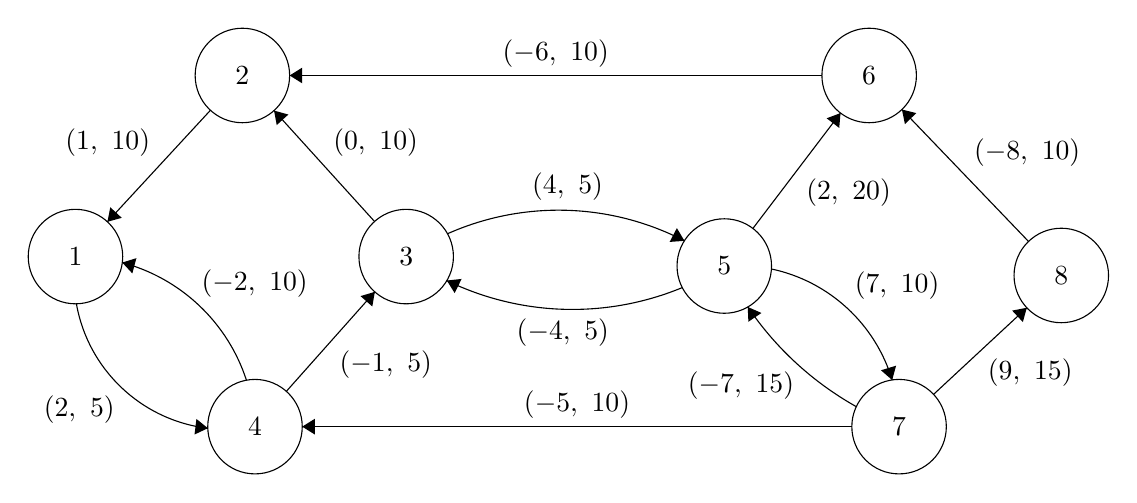
\begin{tikzpicture}[scale=0.2]
            \tikzstyle{every node}+=[inner sep=0pt]
            \draw [black] (7.5,-23.2) circle (3);
            \draw (7.5,-23.2) node {$1$};
            \draw [black] (18.1,-11.7) circle (3);
            \draw (18.1,-11.7) node {$2$};
            \draw [black] (28.5,-23.2) circle (3);
            \draw (28.5,-23.2) node {$3$};
            \draw [black] (18.9,-34) circle (3);
            \draw (18.9,-34) node {$4$};
            \draw [black] (48.7,-23.8) circle (3);
            \draw (48.7,-23.8) node {$5$};
            \draw [black] (57.9,-11.7) circle (3);
            \draw (57.9,-11.7) node {$6$};
            \draw [black] (59.8,-34) circle (3);
            \draw (59.8,-34) node {$7$};
            \draw [black] (70.1,-24.4) circle (3);
            \draw (70.1,-24.4) node {$8$};
            \draw [black] (16.07,-13.91) -- (9.53,-20.99);
            \fill [black] (9.53,-20.99) -- (10.44,-20.74) -- (9.71,-20.07);
            \draw (12.27,-15.99) node [left] {$(1,\mbox{ }10)$};
            \draw [black] (26.49,-20.97) -- (20.11,-13.93);
            \fill [black] (20.11,-13.93) -- (20.28,-14.85) -- (21.02,-14.18);
            \draw (23.84,-15.99) node [right] {$(0,\mbox{ }10)$};
            \draw [black] (15.914,-34.105) arc (-96.88988:-170.01381:9.662);
            \fill [black] (15.91,-34.1) -- (15.18,-33.51) -- (15.06,-34.5);
            \draw (7.74,-32.01) node [below] {$(2,\mbox{ }5)$};
            \draw [black] (10.467,-23.582) arc (75.10435:17.99197:11.37);
            \fill [black] (10.47,-23.58) -- (11.11,-24.27) -- (11.37,-23.3);
            \draw (18.88,-25.83) node [above] {$(-2,\mbox{ }10)$};
            \draw [black] (20.89,-31.76) -- (26.51,-25.44);
            \fill [black] (26.51,-25.44) -- (25.6,-25.71) -- (26.35,-26.37);
            \draw (24.24,-30.05) node [right] {$(-1,\mbox{ }5)$};
            \draw [black] (31.123,-21.751) arc (113.97014:62.62715:17.372);
            \fill [black] (46.17,-22.2) -- (45.69,-21.39) -- (45.23,-22.27);
            \draw (38.75,-19.68) node [above] {$(4,\mbox{ }5)$};
            \draw [black] (46.034,-25.169) arc (-67.52021:-115.8825:18.262);
            \fill [black] (31.08,-24.72) -- (31.58,-25.52) -- (32.02,-24.62);
            \draw (38.45,-27.14) node [below] {$(-4,\mbox{ }5)$};
            \draw [black] (56.8,-34) -- (21.9,-34);
            \fill [black] (21.9,-34) -- (22.7,-34.5) -- (22.7,-33.5);
            \draw (39.35,-33.5) node [above] {$(-5,\mbox{ }10)$};
            \draw [black] (54.9,-11.7) -- (21.1,-11.7);
            \fill [black] (21.1,-11.7) -- (21.9,-12.2) -- (21.9,-11.2);
            \draw (38,-11.2) node [above] {$(-6,\mbox{ }10)$};
            \draw [black] (50.52,-21.41) -- (56.08,-14.09);
            \fill [black] (56.08,-14.09) -- (55.2,-14.42) -- (56,-15.03);
            \draw (53.87,-19.15) node [right] {$(2,\mbox{ }20)$};
            \draw [black] (68.02,-22.24) -- (59.98,-13.86);
            \fill [black] (59.98,-13.86) -- (60.17,-14.79) -- (60.89,-14.09);
            \draw (64.53,-16.58) node [right] {$(-8,\mbox{ }10)$};
            \draw [black] (61.99,-31.95) -- (67.91,-26.45);
            \fill [black] (67.91,-26.45) -- (66.98,-26.63) -- (67.66,-27.36);
            \draw (68.13,-29.68) node [below] {$(9,\mbox{ }15)$};
            \draw [black] (51.684,-23.985) arc (78.06152:16.7775:10.233);
            \fill [black] (59.36,-31.04) -- (59.61,-30.13) -- (58.65,-30.42);
            \draw (59.67,-25.98) node [above] {$(7,\mbox{ }10)$};
            \draw [black] (57.085,-32.731) arc (-119.27953:-145.88145:20.339);
            \fill [black] (50.19,-26.4) -- (50.23,-27.34) -- (51.06,-26.78);
            \draw (49.76,-30.45) node [below] {$(-7,\mbox{ }15)$};
          \end{tikzpicture}
        \end{center}
      \item
        The node potentials must satisfy the following set of equations:\\
        \begin{equation}
          \begin{split}
            1-\pi_2+\pi_1&\geq0\\
            -\pi_2+\pi_3&=0\\
            1-\pi_3+\pi_4&=0\\
            2-\pi_1+\pi_4&=0\\
            6-\pi_2+\pi_6&=0\\
            4-\pi_3+\pi_5&=0\\
            5-\pi_4+\pi_7&=0\\
            2-\pi_5+\pi_6&\geq0\\
            7-\pi_5+\pi_7&=0\\
            9-\pi_7+\pi_8&\geq0\\
            8-\pi_6+\pi_8&=0\\
          \end{split}
        \end{equation}
        Did not finish. Octave is telling me this set of equations is unsatisfiable.
      \item Did not finish.
    \end{enumerate}
  % #5
  \item
    \begin{enumerate}
      \item Consider: 0 0 2 1.\\
      If Alice goes first, she loses. She will pick the 1, allowing Bob to pick
      the 2. Then her and Bob will split the remaining 0`s. If Bob goes first,
      he can pick the 0, and then this is no different from Alice going first.
      \item
        Assume that Alice will move first.\\
        Define $V(c,i,j,t)=\begin{cases}
          0 &\mbox{if}\ i\geq j\\
          \max(c_i + V(c,i+1,j,!t), c_{j-1}+V(c,i,j-1,!t)) &\mbox{if}\ t\\
          \min(-c_i + V(c,i+1,j,!t), -c_{j-1}+V(c,i,j-1,!t)) &\mbox{otherwise}\end{cases}$
        \begin{algorithm}
          \caption{Gambling Strategy for Alice, DP approach}
          \begin{algorithmic}[1]
            \State \textbf{Input} $C\gets$ array of chips; length $n$
            \State $V\gets$ $n\times n+1$ matrix
            \State Initialize $V_{ij}\gets0$, for $i\geq j$
            \State $turn\gets n\mod2=0$ //{true if Alice's turn (maximization), false otherwise (minimization)}\\
            \For{$diag\gets1\ldots n$}
              \For{$j\gets diag\ldots n+1$}
                \For{$i\gets0\ldots n-diag$}
                  \If{$turn$}
                    \State $V_{ij}=\max(C_i + V_{i+1,j},C_{j-1} + V_{i,j-1})$
                  \Else
                    \State $V_{ij}=\min(-C_i + V_{i+1,j},-C_{j-1} + V_{i,j-1})$
                  \EndIf
                  \State // Note: Also record backpointer to the argmax/argmin
                \EndFor
              \EndFor
            \EndFor
            \State
            \Return Path from following backpointers starting from $V_{0,n+1}$
          \end{algorithmic}
        \end{algorithm}

        So, to use shortest paths, when constructing the $V$ matrix, simply reverse
        the pointers that are being constructed, then compute the shortest path from
        each point along the $i=j$ diagonal, and choose the maximum.

      \item
        The running time of the DP approach is $O(n^2)$. The running time of the
        shortest path approach is also $O(n^2\log n)$ ($n^2$ to build the matrix,
        as in the DP approach but then $n\log n$ for each node along the diagonal).\\
        This can be improved upon by computing intermediate shortest paths while
        constructing the graph, which is what the dynamic programming approach does.\\
    \end{enumerate}
  % #6
  \item Postponed.
  % #7
  \item
    Beginning with the linear program:\\
    \begin{equation}
      \begin{split}
        \text{min}\ &x_1+x_2+3x_3+2x_4+4x_5\\
        \text{s.t.}\ &x_1+x_3+x_5=2\\
        &x_4-x_3=1\\
        &x_2-x_1=-1\\
        &-x_2-x_4-x_5=-2\\
        &0\leq x_1\leq1\\
        &0\leq x_2\leq2\\
        &0\leq x_3\leq1\\
        &0\leq x_4\leq3\\
        &0\leq x_5\leq2\\
      \end{split}
    \end{equation}
    (I inverted the last equality constraint, but this is the same problem).\\
    The four equality constraints correspond to the four nodes (and their supplies/demands)
    in the network, and the inequality constraints correspond to the lower and upper bounds
    of the arcs in the network.\\
    So we have the following equivalent network (each arc is $(c,l,u)$:\\
    \begin{center}
      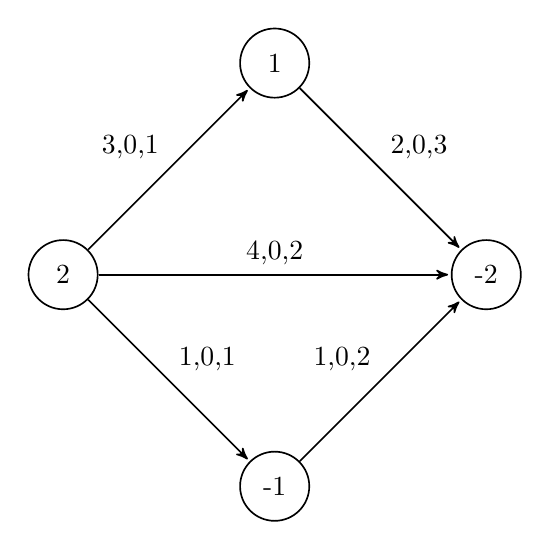
\begin{tikzpicture}[->,>=stealth',shorten >=1pt,auto,node distance=3.8cm,semithick]
        \node[state] (A) {2};
        \node[state] (B) [above right of=A] {1};
        \node[state] (C) [below right of=A] {-1};
        \node[state] (D) [below right of=B] {-2};

        \path (A) edge node {3,0,1} (B) % x_3
                  edge node {1,0,1} (C) % x_1
                  edge node {4,0,2} (D) % x_5
              (B) edge node {2,0,3} (D) % x_4
              (C) edge node {1,0,2} (D) % x_2
              ;
      \end{tikzpicture}
    \end{center}

    Now, we have a MCNF problem with all lower and upper bounds integer, and supplies
    and demands integer. So without loss of generality, this problem has an integer
    solution which is optimal.\\
\end{enumerate}
\end{document}
